\documentclass[a4paper,12pt,fleqn,oneside]{article} 
%\documentclass[a4paper,12pt,fleqn,oneside]{article} 	% Openright aabner kapitler paa hoejresider (openany begge)

%===== Projekt konstanter =====
\newcommand{\kursusTitel}{Semesterprojekt 3}
\newcommand{\linje}{E/IKT}
\newcommand{\semester}{3}
\newcommand{\system}{Beer Pong Table}
\newcommand{\rapportType}{Proces}
\newcommand{\gruppeNr}{7}
\newcommand{\vejleder}{Martin Ansbjerg Kjaer}
\newcommand{\afleveringsdato}{19. december 2018}

%%%% PAKKER %%%%
% ¤¤ Oversaettelse og tegnsaetning ¤¤ %
\usepackage[utf8]{inputenc}					% Input-indkodning af tegnsaet (UTF8)
\usepackage[english, danish]{babel}			% Dokumentets sprog
\usepackage[T1]{fontenc}					% Output-indkodning af tegnsaet (T1)
\usepackage{ragged2e,anyfontsize}			% Justering af elementer

% ¤¤ Figurer og tabeller (floats) ¤¤ %
\usepackage{wrapfig}                        % text wrapping
\usepackage{graphicx} 						% Haandtering af eksterne billeder (JPG, PNG, PDF)
\usepackage{caption}
\usepackage{subcaption}
\usepackage{multirow}
% Fletning af raekker og kolonner (\multicolumn og \multirow)
\usepackage{makecell}                       % Line breaks i tabelceller med \makecell{bla bla \\ bla bla}
\usepackage{colortbl} 						% Farver i tabeller (fx \columncolor, \rowcolor og \cellcolor)
\usepackage[dvipsnames,table,longtable,x11names]{xcolor}

%Tabel automatisk ny linje
\usepackage{array}
\newcolumntype{L}[1]{>{\raggedright\let\newline\\\arraybackslash\hspace{0pt}}m{#1}}
\newcolumntype{C}[1]{>{\centering\let\newline\\\arraybackslash\hspace{0pt}}m{#1}}
\newcolumntype{R}[1]{>{\raggedleft\let\newline\\\arraybackslash\hspace{0pt}}m{#1}}

% Definer farver med \definecolor. Se mere: http://en.wikibooks.org/wiki/LaTeX/Colors
\usepackage{flafter}						% Soerger for at floats ikke optraeder i teksten foer deres reference
\let\newfloat\relax 						% Justering mellem float-pakken og memoir
\usepackage{float}							% Muliggoer eksakt placering af floats, f.eks.
\usepackage{afterpage}
%\usepackage{scrextend}                      % labeling lister
\usepackage{chngcntr} % kontroller nummerering af floats
\counterwithin{figure}{section} % sæt nummerering efter sektion
\counterwithin{table}{section} % sæt nummerering efter sektion

% ¤¤ Matematik mm. ¤¤
\usepackage{amsmath,amssymb,stmaryrd} 		% Avancerede matematik-udvidelser
\usepackage{mathtools}						% Andre matematik- og tegnudvidelser
\usepackage{textcomp}                 		% Symbol-udvidelser (f.eks. promille-tegn med \textperthousand )
\usepackage{siunitx}						% Flot og konsistent praesentation af tal og enheder med \si{enhed} og \SI{tal}{enhed}
\sisetup{output-decimal-marker = {,}}		% Opsaetning af \SI (DE for komma som decimalseparator)

% ¤¤ Misc. ¤¤ %
\usepackage{listings}						% Placer kildekode i dokumentet med \begin{lstlisting}...\end{lstlisting}

%Custom C Code Style
\lstdefinestyle{customc}{
    breaklines=true,
    language=C,
    basicstyle=\small\sffamily,
    numbers=left,
    numberstyle=\tiny\color{gray},
    frame=tb,
    columns=fullflexible,
    showstringspaces=false,
    keywordstyle=\bfseries\color{green!40!black},
    commentstyle=\itshape\color{purple!40!black},
    identifierstyle=\color{blue},
    stringstyle=\color{orange},
}


\usepackage{blindtext}
\usepackage{lipsum}							% Dummy text \lipsum[..]
\usepackage[shortlabels]{enumitem}			% Muliggoer enkelt konfiguration af lister
\usepackage{pdfpages}						% Goer det muligt at inkludere pdf-dokumenter med kommandoen \includepdf[pages={x-y}]{fil.pdf}
\usepackage[bottom]{footmisc}               % Saetter footnotes i bunden af siden
\pdfoptionpdfminorversion=6					% Muliggoer inkludering af pdf dokumenter, af version 1.6 og hoejere
\pretolerance=2500 							% Justering af afstand mellem ord (hoejt tal, mindre orddeling og mere luft mellem ord)


%%%% BRUGERDEFINEREDE INDSTILLINGER %%%%

\linespread{1,1}							% Linie afstand

% ¤¤ Visuelle referencer ¤¤ %
\usepackage[colorlinks,pdfencoding=auto]{hyperref}			% Danner klikbare referencer (hyperlinks) i dokumentet.
\hypersetup{colorlinks = true,				% Opsaetning af farvede hyperlinks (interne links, citeringer og URL)
    linkcolor = black,
    citecolor = black,
    urlcolor = black
}

%%%% TODO-NOTER %%%%
\usepackage[danish, colorinlistoftodos]{todonotes}
%\usepackage[colorinlistoftodos]{todonotes}

%%%% TABEL BAGGRUNDSFARVER %%%%
\definecolor{aublueclassic}{RGB}{0,61,115}
\definecolor{aubluedark}{RGB}{0,37,70}
\definecolor{aucyan}{RGB}{225,248,253}
%\definecolor{aucyan}{RGB}{55,160,203}
\definecolor{aucyandark}{RGB}{0,62,92}
\definecolor{lightGray}{RGB}{153,153,153}
\definecolor{darkGray}{RGB}{119,119,119}
\definecolor{khaki}{RGB}{240,230,140}
\definecolor{lavender}{RGB}{230,230,250}

%indentering af section
\usepackage{changepage}

%Code highlighting
\usepackage{minted}

%%%% Tabs %%%%
\usepackage{tabto}
\NumTabs{10}

%%%% REFERENCE TIL SECTION-NAME %%%%
\usepackage{nameref}
\newcommand*{\fullref}[1]{\textbf{\ref{#1} \nameref{#1}}} % One single link

%sidehoved
\usepackage{fancyhdr}
\usepackage{lastpage}

%referer til afsnit i andre dokumenter
\usepackage{xr}

\externaldocument[arch:]{aux_files/Arkitektur}
\externaldocument[accepttestspec:]{aux_files/Accepttestspecifikation}
\externaldocument[hwdesign:]{aux_files/HardwareDesign}
\externaldocument[analyse:]{aux_files/Analyse}
\externaldocument[integration:]{aux_files/Integrationstest}
\externaldocument[kravspec:]{aux_files/Kravspecifikation}
\externaldocument[modultest:]{aux_files/Modultest}
\externaldocument[proces:]{aux_files/Procesdokument}
\externaldocument[swdesign:]{aux_files/Softwaredesign}

%%%% biblatex %%%%
\usepackage[backend=bibtex,style=ieee]{biblatex}
\bibliography{Litteratur} 

%%%% KRAV numerering %%%%

\newcounter{req} \setcounter{req}{0}
\newcounter{subreq}[req] \setcounter{subreq}{0}
 
\renewcommand{\thereq}{\arabic{req}}
\renewcommand{\thesubreq}{\arabic{req}.\arabic{subreq}}
 
\newenvironment{req}[1]%
{
\refstepcounter{req}{K\thereq}}{}
\newenvironment{subreq}[1]%
{
\refstepcounter{subreq}{\noindent K\thesubreq}}{}


%%%% paragraph %%%%
%\usepackage{titlesec}
%\setcounter{secnumdepth}{4}

%\titleformat{\paragraph}
%{\normalfont\normalsize\bfseries}{\theparagraph}{1em}{}
%\titlespacing*{\paragraph}
%{0pt}{3.25ex plus 1ex minus .2ex}{1.5ex plus .2ex}

% ========== PAKKER DER SKAL LOADES TIL SIDST ==================
%\usepackage{xcolor}
%\usepackage{listings}
\usepackage{csquotes}           %så holder bilatex kæft
\usepackage{subfiles}


%%EDS SHIT
\PassOptionsToPackage{unicode=true}{hyperref} % options for packages loaded elsewhere
\PassOptionsToPackage{hyphens}{url}
%
\usepackage{lmodern}
\usepackage{amssymb,amsmath}
\usepackage{ifxetex,ifluatex}
\ifnum 0\ifxetex 1\fi\ifluatex 1\fi=0 % if pdftex
  \usepackage[T1]{fontenc}
  \usepackage[utf8]{inputenc}
  \usepackage{textcomp} % provides euro and other symbols
\else % if luatex or xelatex
  \usepackage{unicode-math}
  \defaultfontfeatures{Ligatures=TeX,Scale=MatchLowercase}
\fi
% use upquote if available, for straight quotes in verbatim environments
\IfFileExists{upquote.sty}{\usepackage{upquote}}{}
% use microtype if available
\IfFileExists{microtype.sty}{%
\usepackage[]{microtype}
\UseMicrotypeSet[protrusion]{basicmath} % disable protrusion for tt fonts
}{}
\IfFileExists{parskip.sty}{%
\usepackage{parskip}
}{% else
\setlength{\parindent}{0pt}
\setlength{\parskip}{6pt plus 2pt minus 1pt}
}
\usepackage{hyperref}
\hypersetup{
            pdfborder={0 0 0},
            breaklinks=true}
\urlstyle{same}  % don't use monospace font for urls
\usepackage{longtable,booktabs}
% Fix footnotes in tables (requires footnote package)
\IfFileExists{footnote.sty}{\usepackage{footnote}\makesavenoteenv{longtable}}{}
\setlength{\emergencystretch}{3em}  % prevent overfull lines
\providecommand{\tightlist}{%
  \setlength{\itemsep}{0pt}\setlength{\parskip}{0pt}}
% Redefines (sub)paragraphs to behave more like sections
\ifx\paragraph\undefined\else
\let\oldparagraph\paragraph
\renewcommand{\paragraph}[1]{\oldparagraph{#1}\mbox{}}
\fi
\ifx\subparagraph\undefined\else
\let\oldsubparagraph\subparagraph
\renewcommand{\subparagraph}[1]{\oldsubparagraph{#1}\mbox{}}
\fi

% set default figure placement to htbp
\makeatletter
\def\fps@figure{htbp}
\makeatother
\def\titlename{Projektformulering}

% Den oprindelige projektformulering

\begin{document}
\begin{titlepage}

\newcommand{\HRule}{\rule{\linewidth}{0.5mm}} % Defines a new command for the horizontal lines, change thickness here

\center % Center everything on the page
 
%----------------------------------------------------------------------------------------
%	HEADING SECTIONS
%----------------------------------------------------------------------------------------

\textsc{\LARGE Aarhus Universitet }\\[0.3cm] % Name of your university/college
\textsc{\Large 3. Semesterprojekt }\\[0.3cm]
\textsc{\Large Gruppe 7 }\\[0.5cm] % Major heading such as course name
 % Minor heading such as course title

%----------------------------------------------------------------------------------------
%	TITLE SECTION
%----------------------------------------------------------------------------------------

\HRule \\[0.4cm]
{ \huge \bfseries \titlename}\\[0.03cm]{Beerpong Table} % Title of your document
\HRule \\[1.5cm]

 
%----------------------------------------------------------------------------------------
%	AUTHOR SECTION
%----------------------------------------------------------------------------------------

\begin{minipage}{0.4\textwidth}
\begin{flushleft} \small
\emph{Gruppemedlemmer:}
\\Aaron Becerril Sanchez\\ (AU592162)
\\Edward Hestnes Brunton\\ (AU576633)
\\Marcus Gasberg\\ (AU587414) 
\\Martin Gildberg Jespersen\\ (AU593618) 
\\Martin Lundberg\\ () 
\\Mathias Magnild Hansen\\ (AU520773)
\\Nikolaj Holm Gylling\\ (AU592243)
\\Tristan Moeller\\ (AU569046)
\end{flushleft}
\end{minipage}
~
\begin{minipage}{0.4\textwidth}
\begin{flushright} \small
\emph{Vejleder:} \\
Martin Ansbjerg Kjær \\ Civ. Ing., Ph.D., Adjunkt % Supervisor's Name
\end{flushright}
\end{minipage}\\[1cm]

% If you don't want a supervisor, uncomment the two lines below and remove the section above
%\Large \emph{Author:}\\
%John \textsc{Smith}\\[3cm] % Your name

%----------------------------------------------------------------------------------------
%	DATE SECTION
%----------------------------------------------------------------------------------------

{\large December 2018}\\[1cm] % Date, change the \today to a set date if you want to be precise

%----------------------------------------------------------------------------------------
%	LOGO SECTION
%----------------------------------------------------------------------------------------


\includegraphics{Setup/graphics/AU.png}\\[1cm] %Logo

\vfill
\end{titlepage}
\section{Projektformulering}
\subsection{Indledning}
Målet for dette projekt er at udarbejde et Beer pong bord. Beer pong er et populært drukspil, som typisk spilles af to konkurrerende hold af 2-4 spillere. Spillerne står på hver deres side af bordet og kaster på skift en bordtennisbold hen over bordet, med hensigten at ramme ned i modstanderens øl kop i den anden ende. Øl kopperne placeres typisk i en trekantet formation af 6 kopper i hver ende af bordet, og holdene skiftes til at kaste bolden. Når bolden lander i en kop, indtages indholdet af modstanderen og koppen fjernes fra bordet. Vinderen er det hold, som først eliminerer alle modstanderens kopper. 
På trods af at spillet er populært og udbredt, foregår langt de fleste spil på simple og inferiøre borde. Ofte er der delte meninger omkring spillets score, hvis tur det er til at kaste og om legitimiteten af de enkelte kast. Derudover kan kopper vælte og indholdet spildes. Det resulterer ofte i udbredt forvirring og en forringet brugeroplevelse.  Ved at udvikle en forbedret og interaktiv udgave af et Beer pong bord, sikres en mere underholdende og komplet oplevelse for spillerne, og forvirringen minimeres. En skitse af opstillingen ses nedenfor.
\begin{figure}[H]
    \centering
    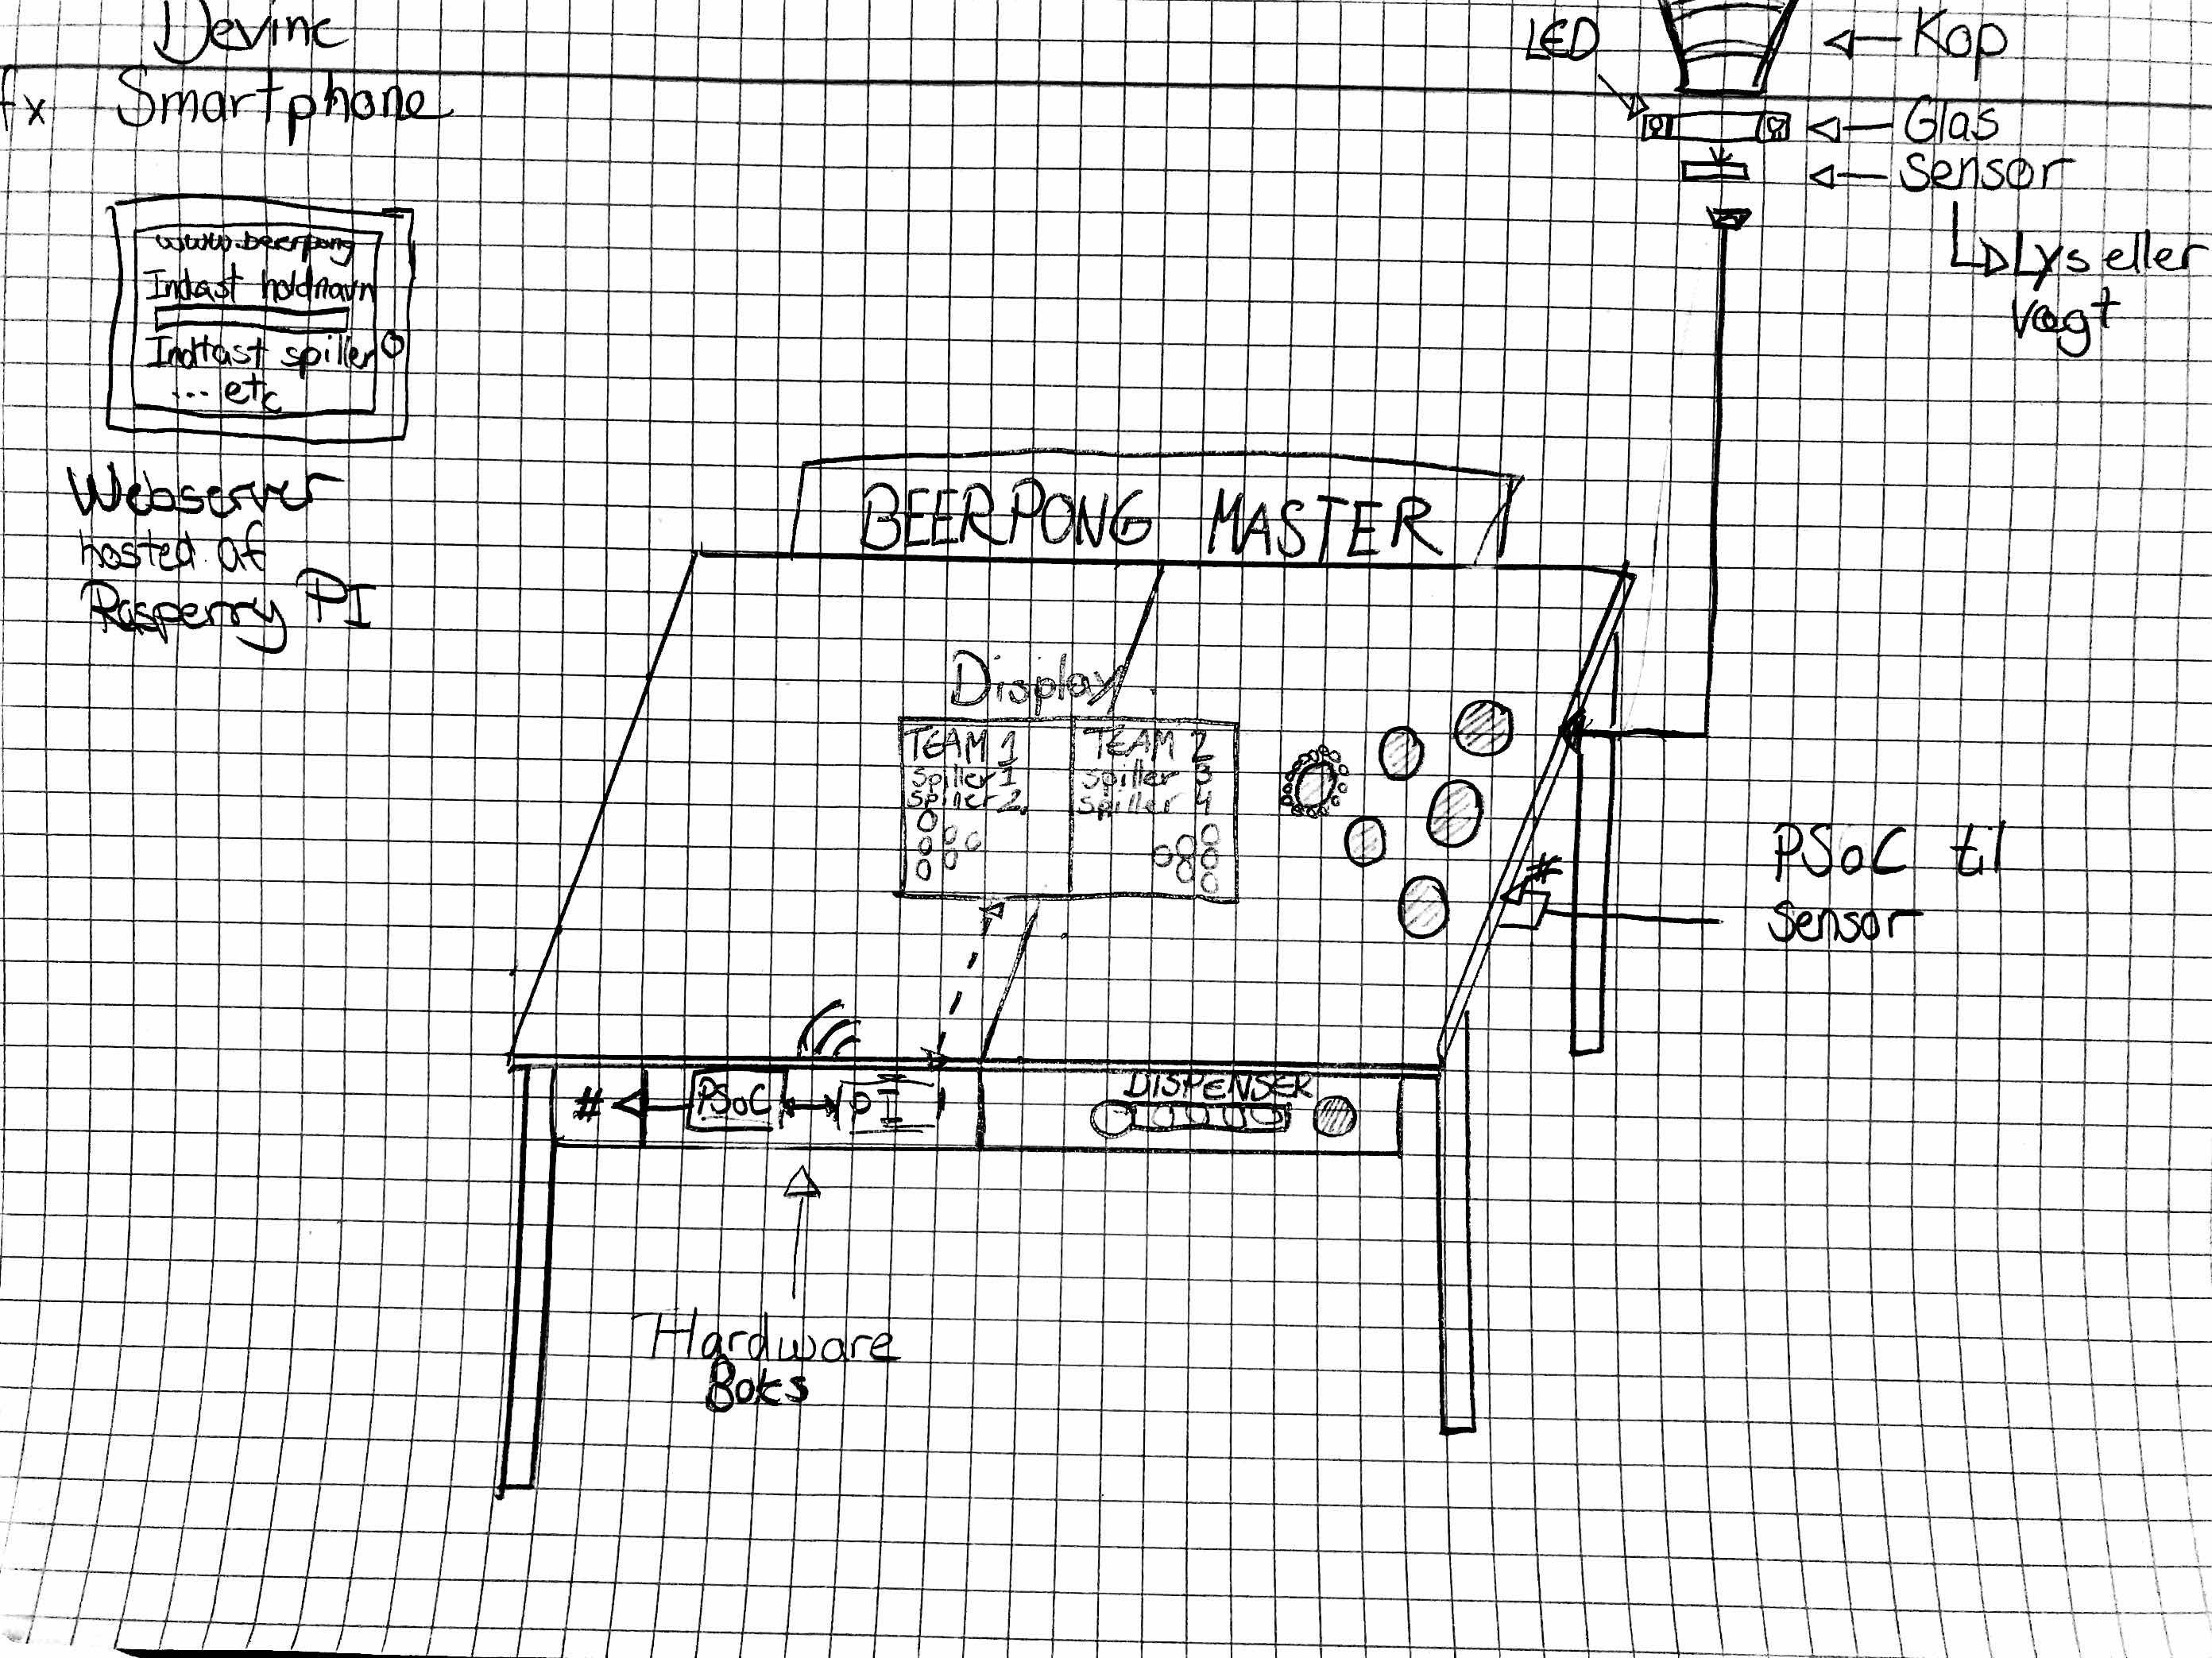
\includegraphics[width=\textwidth]{Projektformulering/graphics/BeerPong_oprindelig_skitse.png}
    \caption{Skitse af Beer Pong Table}
    \label{fig:ShiftRegPWM_test}
\end{figure}
\subsection{Problemformulering}
I dette projekt udvikles og designes et interaktivt Beer pong bord, som interagerer ud fra brugerens adfærd. I et traditionelt spil Beer pong er det spillerens ansvar at styre spillets gang. Der ønskes et system, som automatiserer spillets gang og underholder med et interaktiv design. 

Fra et mobilt device - f.eks. en smartphone - skal brugeren kunne indtaste hvilke spillere, som skal deltage i spillet og hvilke hold de skal høre under. Denne information skal opdateres på et display, som er placeret på midten af Beerpong-bordet. Efter spillet er startet skal systemet agerer ud fra spillets gang. Når en spiller fjerner en kop, skal en sensor registrere dette og opdatere displayet. Her kan der også laves en timer, der begynder ved registrering af at et glas er løftet og kan evt. bruges ved en challenge*. Der kan også med fordel implementeres et system til at registrere, at en bold rammer ned i en kop. Dermed kan spillerne få visuel eller auditiv feedback med det samme i tilfælde af et succesfuldt kast. 
Den visuelle feedback kommer fra belysning under kopperne, men det kan udvides til at have belysning rundt om hele bordet. Displayet skal være spillere og tilskueres adgang til information om spillet. Det skal angive antallet af kopper, der er tilbage på bordet, spillerne og holdenes navne.  

Det er et krav til denne opgave, at systemet skal etableres ved en indlejret Linux platform og en PSoC platform. Desuden skal systemet kunne interagere med omverdenen via sensorer/aktuatorer. Her inkluderes en dispenser i spillet, der ved hjælp af en aktuator forsyner spillere med bordtennisbolde ved indsætning af mønter.

Det endelige produkt af projektet skal være en prototype, der demonstrerer, at ovenstående kan realiseres. 
\subsection{MoSCoW}
\begin{table}[H]
\begin{tabular}{|l|l|}
\hline
\textbf{Must have} & \begin{tabular}[c]{@{}l@{}}- 6 kopholdere\\ - Belysning under/rundt om hver kop\\ - Registrering af fjernelse af kop fra bord\\ - Dispenser til Bordtennisbold\\ - Registrer mønter til at dispensere bordtennisbolde\\ - UI til visning af scoreboards, holdet og hvis tur det er\end{tabular} \\ \hline
\textbf{Should have} & \begin{tabular}[c]{@{}l@{}}- 12 kopholdere(6 for hver side) \\ - Indtastning af information fra mobilt device \\ - Registrering at et glas er blevet ramt af bold \\ (og giver visuelt/auditivt respons)\\ - Ved fjernelse af kop udløses timer, som \\ kan stoppes ved tryk på knap\end{tabular} \\ \hline
\textbf{Could have} & \begin{tabular}[c]{@{}l@{}}- Hjemmeside til at gemme resultater fra forskellige spil\\ - Belysning rundt om bordet\end{tabular} \\ \hline
\textbf{Wont have} & \begin{tabular}[c]{@{}l@{}}- Bevægende ringe på midten af banen til at kaste bolde \\ igennem(for eksempel som en challenge*)\end{tabular} \\ \hline
\end{tabular}
\end{table}
*challenge=En udfordring, som for eksempel at bunde en øl hurtigere end det andet hold












\end{document}